% Compiler Pass Ordering with Sequence-Aware Bayesian Optimization
% Self-contained manuscript: compiles on Overleaf (pdfLaTeX) with no extra class files.
% To use the official IEEE Access template instead, see ../README.md ("Manuscript").
\documentclass[10pt,twocolumn]{article}
\usepackage[a4paper,margin=0.75in,columnsep=0.25in]{geometry}
\usepackage{amsmath,amssymb}
\usepackage{booktabs,tabularx,array}
\usepackage{graphicx}
\usepackage{enumitem}
\usepackage{algorithm}
\usepackage{tikz}
\usetikzlibrary{arrows.meta,positioning,shapes.geometric}
\usepackage{microtype}
\usepackage[hidelinks]{hyperref}
\usepackage{titlesec}
\usepackage{caption}
\captionsetup{font=small,labelfont=bf,labelsep=period}
\titleformat{\section}{\normalsize\bfseries\centering}{\Roman{section}.}{0.5em}{\MakeUppercase}
\titleformat{\subsection}{\normalsize\bfseries}{\Alph{subsection}.}{0.5em}{}
\renewcommand{\thetable}{\arabic{table}}
\renewcommand{\thefigure}{\arabic{figure}}

% --- helpers used in sections/related_work.tex --------------------------------
\newcounter{study}
\makeatletter
\@addtoreset{study}{subsection}
\makeatother
\newcommand{\study}[1]{\par\medskip\refstepcounter{study}\noindent\textbf{\thestudy)\ #1}\par\smallskip}
\newcommand{\ps}{\textbf{Proposed solution:}}
\newcommand{\me}{\textbf{Methodology:}}
\newcommand{\re}{\textbf{Results:}}
\newcommand{\rg}{\textbf{Research gap:}}
\newenvironment{IEEEkeywords}{\par\smallskip\noindent\textbf{INDEX TERMS}\ \itshape}{\par}

\title{\textbf{Compiler Pass Ordering with\\ Sequence-Aware Bayesian Optimization}}
\author{%
Shaurya Raghav, Manyata Tripathi, Yakshith Reddy, Piyush Mahto, and Bhuvaneswari M\\[2pt]
\small School of Computer Science and Engineering, Vellore Institute of Technology, Vellore, Tamil Nadu, India\\
\small Corresponding author: Bhuvaneswari M (e-mail: m.bhuvaneswari@vit.ac.in)}
\date{}

\begin{document}
\twocolumn[\maketitle\begin{abstract}
Compiler optimization can significantly influence program execution time, yet determining an effective ordering of optimization passes remains challenging because the impact of a pass depends on the sequence in which transformations are applied. This work investigates sequence-aware Bayesian optimization for compiler pass ordering using the LLVM compilation framework. The proposed approach uses a Gaussian Process surrogate with a sequence-aware kernel, Expected Improvement for candidate selection, and warm-start information across benchmark programs. It is compared with Random Search, a Genetic Algorithm, Tree-structured Parzen Estimator (TPE) optimization, and a variant without warm start on five PolyBench/C benchmarks, using 20 evaluations per search and five random seeds. After correctness checking and re-timing, the geometric-mean speedup relative to LLVM \texttt{-O3} is 0.942 for the proposed method, 0.952 for TPE, 0.947 for Random Search, and 0.917 for the Genetic Algorithm. Paired Wilcoxon tests show no significant difference in verified speedup between the proposed method and any other method (all $p > 0.3$), and removing the warm start does not change the result. No method matches \texttt{-O3} on average. In exploratory comparisons of search cost, the proposed method produced fewer failed builds than TPE and spent less time per search than all baselines, mainly because its candidates executed faster. Its verified performance advantage therefore remains unproven under this budget.
\end{abstract}
\begin{IEEEkeywords}
Bayesian optimization, compiler autotuning, compiler optimization, LLVM, optimization pass ordering, program performance.
\end{IEEEkeywords}
\vspace{4pt}]
\section{Introduction}
Compiler optimization is an essential stage in translating high-level programs into efficient executable code. Modern compilers apply a sequence of transformations to an intermediate representation to improve execution time, reduce code size, and exploit hardware resources. However, the effectiveness of an optimization pass depends not only on the transformation itself but also on the transformations that precede and follow it. Consequently, selecting an effective ordering of compiler optimization passes is a challenging search problem \cite{ashouri2018survey,nobre2019nonio,kruse2020autotuning,queiroz2020hybrid,liu2024dco}.

LLVM provides a flexible compilation framework in which optimization passes can be composed into pipelines. Although standard optimization levels such as \texttt{-O3} provide strong general-purpose performance, a fixed pipeline may not be optimal for every program. Different applications exhibit different computational characteristics, and interactions between passes can produce different performance outcomes. Exhaustively evaluating every possible pass sequence is impractical because the search space grows rapidly with sequence length \cite{trofin2021mlgo,cummins2022compilergym,ashouri2024acpo}.

Search-based methods provide an alternative to exhaustive evaluation. Random search samples candidate sequences without learning from earlier evaluations, while genetic algorithms use population-based evolutionary operations. Reinforcement-learning approaches have also been investigated for compiler phase ordering, including LLVM-based optimization and high-level synthesis. These approaches demonstrate both the potential and the workload dependence of learned pass sequences \cite{hajali2020autophase,wu2020roicf,jain2022poset,shahzad2022rl}.

This work investigates a sequence-aware Bayesian optimization approach for LLVM compiler pass ordering. The proposed method uses a Gaussian Process surrogate with a sequence-aware kernel, Expected Improvement for candidate selection, and warm-start information across benchmark programs. Its performance is compared with Random Search, a Genetic Algorithm, Tree-structured Parzen Estimator (TPE), and a no-warm-start ablation using five PolyBench/C benchmarks. Recent compiler autotuning and pass-ordering studies provide relevant comparison points for this evaluation \cite{pouchet2016polybench,wu2022bayesian,liang2023coreset,ashouri2022mlgoperf,chang2023ensemble}.

The main contributions of this work are:
\begin{enumerate}[leftmargin=*,itemsep=1pt]
\item An experimental framework for evaluating candidate LLVM pass sequences through compilation, runtime measurement, and correctness checking.
\item A comparative evaluation of four search strategies, together with a no-warm-start ablation, under a limited budget of 20 evaluations per search.
\item An analysis of runtime speedup, tuning cost, compilation overhead, and variability across five benchmark programs, including the distinction between search-time results and final verified results.
\end{enumerate}
The remainder of this paper presents related work, the problem formulation and proposed method, the experimental setup, results, limitations, and future work.

\section{Related Work}
Compiler optimization pass ordering, also known as the phase-ordering problem, concerns selecting not only which transformations to apply but also the order in which they are applied. The effects of individual passes may depend on the intermediate representation produced by previous transformations. Consequently, an effective optimization strategy for one program may not provide the same benefit for another program. A survey of machine-learning-based compiler autotuning reviews these challenges and the broader use of learned methods for optimization selection and phase ordering \cite{ashouri2018survey}.

A related direction is to reuse knowledge from previously evaluated programs rather than restarting every search from scratch. Collaborative filtering has been investigated as a way to reuse compiler-optimization measurements across programs and reduce the number of required compilation and performance-test iterations \cite{cereda2020collab}. This motivates the use of cross-program information when constructing initial candidates.

Bayesian optimization has been applied to compiler autotuning, including LLVM Clang/Polly loop-optimization pragmas \cite{wu2022bayesian}. Practical optimization platforms such as Optuna provide configurable samplers and an experimental framework for automated search \cite{akiba2019optuna}. These approaches provide relevant context for comparing model-guided search with random and evolutionary baselines under a limited evaluation budget.

LLVM-based learning frameworks and compiler optimization environments provide the infrastructure needed to train and evaluate learned compiler decisions \cite{trofin2021mlgo,cummins2022compilergym}. The PolyBench/C suite supplies the numerical kernels used in the present evaluation \cite{pouchet2016polybench}. Building on this background, the following studies cover modular autotuning, reinforcement learning, learned compiler decisions, sequence reuse, and dependence-based optimization.

\study{Nonio: Modular Compiler Phase Ordering}
\ps{} Nobre et al.\ introduced Nonio, a modular framework for exploring compiler flags and optimization sequences in modern compilers \cite{nobre2019nonio}.

\me{} The framework supports GCC and Clang/LLVM through an extensible software architecture. Its components allow researchers to integrate different exploration algorithms, objective functions, and compiler toolchains without redesigning the entire system.

The authors demonstrate its use in exploring custom compiler configurations for a C program, considering execution time and energy consumption against standard compiler optimization settings.

\re{} The work demonstrates how a common framework can support compiler design-space exploration and optimization-sequence specialization. Its modular approach makes it useful for comparing optimization strategies.

\rg{} The framework does not specifically establish the effectiveness of a Gaussian Process with a sequence-aware kernel and cross-program warm starts.

\study{Autotuning Search Space for Loop Transformations}
\ps{} Kruse et al.\ proposed a tree-structured representation of loop-transformation configurations to model their relationships more explicitly than a flat parameter vector \cite{kruse2020autotuning}.

\me{} The authors construct a search space that represents loop transformations and their legal relationships. They implement an autotuning system and evaluate it on selected PolyBench kernels, using compiler transformations and performance measurements to explore candidate configurations.

Their design allows transformation sequences to be represented systematically, including complex loop transformations such as multilevel tiling. The experiments also discuss the need for search algorithms capable of navigating this structured space efficiently.

\re{} The study demonstrates how a structured search space can represent loop-transformation configurations. Its findings motivate more effective exploration strategies for complex optimization choices.

\rg{} The work focuses on loop-transformation configurations rather than a general fixed-length sequence of LLVM optimization passes.

\study{Finding Effective Compiler Optimization Sequences: A Hybrid Approach}
\ps{} Queiroz Junior et al.\ proposed a hybrid approach combining machine learning with iterative compilation to address the compiler optimization-selection problem \cite{queiroz2020hybrid}.

\me{} The framework combines predictions from machine-learning techniques with empirical compilation and execution measurements. Rather than relying exclusively on a learned model or an unguided search, it uses their complementary strengths to identify promising optimization configurations.

The authors investigate multiple strategies, evaluation metrics, and hardware platforms. Their experimental design examines how the hybrid method behaves under different optimization scenarios.

\re{} The authors report that the hybrid approach improves on the evaluated machine-learning and iterative compilation alternatives and outperforms the best tested LLVM optimization level.

\rg{} The reported hybrid approach does not specifically investigate the proposed sequence-aware Gaussian Process kernel and Expected Improvement strategy used in this work.

\study{Bayesian Autotuning of PolyBench Programs}
\ps{} Wu et al.\ developed a Bayesian-optimization-based autotuning framework for LLVM Clang/Polly loop-optimization pragmas \cite{wu2022bayesian}.

\me{} The framework, based on the ytopt autotuning system, explores the parameter space of loop-optimization configurations. It evaluates several supervised-learning methods within Bayesian optimization and applies the framework to six computationally intensive PolyBench benchmarks.

The experiments use large benchmark datasets and compare optimization configurations through execution-time measurements. The authors also investigate alternative tuning strategies for cases where the initial autotuning method does not improve performance.

\re{} Their approach identifies lower execution times for five of the six studied benchmarks using 200 evaluations, while Floyd--Warshall does not benefit from the same autotuning configuration.

\rg{} The study primarily tunes loop pragmas and their parameters rather than the ordering of a general set of compiler passes.

\subsection{Reinforcement Learning for Compiler Phase Ordering}
\study{AutoPhase: Learning Phase Orders for High-Level Synthesis}
\ps{} Haj-Ali et al.\ proposed AutoPhase, which combines deep reinforcement learning with program-feature information to discover effective compiler optimization sequences for high-level synthesis (HLS) \cite{hajali2020autophase}.

\me{} The framework applies reinforcement learning in an LLVM-based compilation environment targeting hardware generated through HLS. Random-forest models estimate relationships between program features and the effectiveness of optimization passes, helping reduce the candidate search space.

The authors compare their method with existing phase-ordering approaches and study whether policies trained on a limited set of programs can generalize to additional programs.

\re{} The reported experiments show a 28\% improvement in circuit performance over the \texttt{-O3} baseline. The approach also reports generalization to more than 12,000 programs after training on approximately 100 programs.

\rg{} Its principal target is circuit performance in HLS, which differs from directly minimizing execution time for general-purpose CPU programs.

\study{Reliable Compilation Optimization Sequence Generation}
\ps{} Wu et al.\ introduced ROICF, a reinforcement-learning-based framework for generating reliable compiler optimization sequences \cite{wu2020roicf}.

\me{} The framework is based on the standard LLVM optimization passes and formulates sequence generation as a learning problem. It aims to identify program-specific phase orderings while accounting for compilation reliability.

Wu et al.\ propose ROICF, a reinforcement-learning framework that represents compiler optimization choices as agent actions and uses feedback from compilation to learn program-specific optimization sequences. Its stated emphasis is compilation reliability, so its objective and success criteria differ from runtime-focused comparison.

\re{} The study presents a framework for generating optimization sequences with reliability as an explicit concern. It highlights that the effectiveness of an optimization sequence must be considered together with the reliability of the resulting compilation.

\rg{} ROICF emphasizes compilation reliability, whereas this study evaluates verified runtime speedup under a fixed search budget. A direct performance comparison would require a shared runtime-tuning and verification protocol.

\study{Reinforcement Learning Strategies for Compiler Optimization in HLS}
\ps{} Shahzad et al.\ investigated several reinforcement-learning design choices for compiler optimization in high-level synthesis \cite{shahzad2022rl}.

\me{} The study examines how pass-order information can be incorporated into the agent state, how multiple actions can be grouped into action tuples, and how episode length affects the learning process. It also investigates applying the LLVM \texttt{-O3} backend during training.

These strategies are evaluated in an HLS compilation workflow, where the quality of generated hardware depends on the applied compiler transformations. The work emphasizes the interaction between state representation, action selection, and optimization-sequence construction.

\re{} The study provides an experimental investigation of alternative reinforcement-learning configurations for compiler optimization. It emphasizes that the learning strategy and representation of pass choices are important design decisions.

\rg{} The method is tailored to the HLS setting and does not establish which search strategy is most effective for a small, fixed runtime-tuning budget on CPU benchmarks.

\study{POSET-RL: Optimizing Size and Execution Time}
\ps{} Jain et al.\ developed POSET-RL, a reinforcement-learning approach to phase ordering that targets both executable size and execution time \cite{jain2022poset}.

\me{} The system is integrated with LLVM and models optimization sequences using either manually organized subsequences or subsequences derived from an Oz optimization-dependence graph. Program states are represented using IR2Vec embeddings, which provide information about the intermediate representation.

The approach constructs candidate sequences from optimization subsequences and uses reward information relating to binary size and execution time. Its evaluation includes x86 and AArch64 architectures and programs from SPEC CPU2006, SPEC CPU2017, and MiBench.

\re{} The authors report average improvements of 6.19\% in binary size and 11.99\% in execution time over the Oz sequence for SPEC CPU2017 benchmarks.

\rg{} POSET-RL relies on reinforcement-learning policies and constructed subsequences rather than the probabilistic sequence-similarity model used by the proposed method.

\study{Ensemble Reinforcement Learning for Runtime Memory Optimization}
\ps{} Chang and Park proposed an ensemble reinforcement-learning approach to search for compiler optimization sequences that reduce runtime memory profiles \cite{chang2023ensemble}.

\me{} The work formulates compiler optimization as a sequence-search problem and explores an ensemble of reinforcement-learning strategies. Its target is the memory behavior of compiled programs, which may be particularly important for embedded and resource-constrained applications.

Chang and Park extract 50 LLVM IR program features, reduce feature dimensionality using principal component analysis (PCA), and train an ensemble of reinforcement-learning models on clusters formed from randomly generated programs. Their objective is runtime memory-profile reduction rather than execution-time minimization.

\re{} The work-in-progress report describes a 37\% greater memory-profile reduction than the standard optimization option. Because the objective is memory-profile reduction rather than execution-time minimization, this result is not directly comparable to the speedup values reported in this paper.

\rg{} The work focuses on memory-oriented optimization and does not establish performance under the same runtime objective, search budget, and verification protocol used in this paper.

\subsection{Machine Learning Frameworks and Compiler Infrastructure}
\study{MLGO: Machine Learning-Guided Compiler Optimization}
\ps{} Trofin et al.\ introduced MLGO, a framework for integrating machine-learning-based decision-making into LLVM optimization passes \cite{trofin2021mlgo}.

\me{} The framework replaces selected hand-crafted compiler heuristics with learned models. The authors demonstrate the approach on inlining-for-size optimization, using policy-gradient and evolution-strategy methods to train models and integrate them into the compiler.

The study investigates model training and deployment on real-world compiler workloads. It also evaluates whether models trained using one corpus continue to perform well across different targets and later versions of the software environment.

\re{} The authors report up to 7\% code-size reduction relative to LLVM \texttt{-Oz} for the inlining-for-size case study and show that the learned model generalizes to diverse real-world targets.

\rg{} MLGO demonstrates learning inside individual compiler decisions rather than searching arbitrary pass sequences with a sequence-aware Gaussian Process.

\study{MLGOPerf: An ML-Guided Inliner for Performance}
\ps{} Ashouri et al.\ proposed MLGOPerf, which extends ML-guided inlining toward optimizing execution performance rather than focusing solely on code size \cite{ashouri2022mlgoperf}.

\me{} The framework uses a secondary learned model to estimate the performance reward associated with inlining decisions. This reward supports training a reinforcement-learning agent for performance-oriented function inlining, reducing the need for prohibitively expensive direct performance evaluations during training.

The authors evaluate their approach on SPEC CPU2006 and CBench. They also investigate how improved inlining decisions increase the opportunities for further autotuning of code regions.

\re{} The reported speedups over LLVM \texttt{-O3} reach 1.8\% on SPEC CPU2006 and 2.2\% on CBench. The authors further report up to 26\% more opportunities for region autotuning, potentially enabling additional performance gains.

\rg{} The method focuses on function inlining and its reward model, rather than the complete ordering of a general set of optimization passes.

\study{CompilerGym: A Research Environment for Compiler Optimization}
\ps{} Cummins et al.\ introduced CompilerGym, a reusable environment for studying compiler and program optimization using artificial-intelligence methods \cite{cummins2022compilergym}.

\me{} CompilerGym provides a Gym-style interface through which learning algorithms can interact with compiler tasks using observations, actions, and rewards. The toolkit includes real compiler optimization environments and facilities for conducting repeatable experiments.

The authors characterize the environment's optimization spaces, computational efficiency, and fault tolerance. The infrastructure is designed to reduce the engineering effort needed to compare optimization algorithms and investigate reproducibility issues.

\re{} The publication reports substantially more efficient experimentation than prior approaches, including a 27-fold computational-efficiency improvement in its comparisons, while also addressing fault tolerance and reproducibility.

\rg{} CompilerGym provides experimental infrastructure rather than a single optimization-search algorithm, so it does not by itself resolve the compiler phase-ordering problem.

\subsection{Sequence Reuse and Dependence-Based Optimization}
\study{Learning Compiler Pass Orders Using Coresets}
\ps{} Liang et al.\ proposed learning compiler pass-ordering policies using a small coreset of promising sequences and normalized-value prediction \cite{liang2023coreset}.

\me{} Instead of constructing an entire optimization sequence one pass at a time, the method identifies a compact collection of sequences that perform well across programs. A learned policy predicts normalized values for candidates in this collection and selects sequences for unseen programs.

The experiments cover 4,683 unseen code repositories across 14 datasets. The emphasis is on generalization across program domains and reducing the cost of generating and evaluating complete sequences.

\re{} The authors report an average 4.5\% improvement in code-size optimization relative to LLVM \texttt{-Oz} across the evaluated unseen repositories.

\rg{} The method primarily targets binary size and uses a learned sequence-selection policy rather than Gaussian Process regression for low-budget runtime minimization.

\study{ACPO: An AI-Enabled Compiler Framework}
\ps{} Ashouri et al.\ introduced ACPO, a framework intended to make it easier to integrate machine-learning models into LLVM optimization passes \cite{ashouri2024acpo}.

\me{} The framework supplies Python-based facilities for model training and inference and supports applying learned models to optimization decisions. The authors demonstrate its use with loop-unrolling and function-inlining optimization in LLVM.

The work evaluates learned optimization decisions across PolyBench, Coral-2, CoreMark, Graph500, and CBench. As a work-in-progress publication, it describes a broader integration direction while presenting selected experimental use cases.

\re{} The authors report loop-unrolling improvements over LLVM \texttt{-O3} averaging 4\% on PolyBench, 3\% on Coral-2, 5.4\% on CoreMark, and 0.2\% on Graph500. Combining the inlining and loop-unrolling models yields reported speedups of 4.5\% on PolyBench and 2.4\% on CBench.

\rg{} ACPO supports learned decisions within selected passes, whereas the proposed project investigates search over complete ordered pass sequences.

\study{Dependence-Based Compiler Optimization}
\ps{} Liu et al.\ introduced a dependence-based compiler optimization framework (DCO) that groups related passes into useful subsequences to reduce the phase-ordering search space \cite{liu2024dco}.

\me{} DCO models both source-code dependence and pairwise performance dependence between compiler passes. These relationships are represented using an optimization-dependence graph, which is clustered to generate subsequences intended to preserve beneficial interactions while reducing the number of search choices.

The method is integrated with the OpenTuner and LaMCTS iterative-compilation frameworks and evaluated using CBench and PolyBench. Its experiments investigate runtime performance and code-size optimization across different compiler optimization tasks and hardware platforms.

\re{} The authors report up to 1.22 times the runtime speedup of LLVM \texttt{-O3} and a 1.24-fold improvement in code-size reduction relative to \texttt{-Oz}.

\rg{} DCO relies on dependence graphs and generated subsequences, whereas the proposed method directly models sequence similarity and uses Expected Improvement to guide a limited runtime-search budget.

\subsection{Research Gap and Motivation}
The reviewed studies demonstrate that compiler optimization can be improved through modular design-space exploration, reinforcement learning, machine-learning-guided pass decisions, and dependence-aware sequence construction. They also show that optimization quality depends on the target workload, the objective metric, and the cost of acquiring performance feedback.

However, the reviewed approaches differ in their optimization targets, evaluation budgets, and sequence representations. Several focus on high-level synthesis, code size, loop pragmas, or individual compiler decisions, while other approaches depend on reinforcement-learning training or a predefined collection of subsequences. These differences make it important to compare approaches under a common experimental protocol.

The present work investigates this issue through a controlled comparison of Random Search, a Genetic Algorithm, TPE, and sequence-aware Gaussian Process Bayesian optimization on five PolyBench/C programs. The proposed method represents candidate sequences using position-wise information, ordered adjacent pairs, and pass-content information, then uses Expected Improvement to select candidates for evaluation. Its contribution is an experimental assessment under a restricted budget of 20 evaluations per search, with correctness verification and a distinction between search-time observations and final verified runtime results. Additional work broadens the set of relevant learning and search strategies. Static neural compiler optimization has been studied using deep reinforcement learning, while IR2Vec represents LLVM intermediate representations as scalable program embeddings for machine-learning tasks \cite{mammadli2020static,venkatakeerthy2020ir2vec}. Search guided by learned cost models has also been applied to Halide schedule selection, and transfer-tuning has investigated reusing schedules across related tensor programs to reduce search time \cite{gibson2022transfer,adams2019halide}. Broader surveys and research on machine learning in compiler optimization describe the feature representations, training methods, and deployment challenges involved in learned optimization \cite{wang2018mlcompiler,hajali2021thesis}. More recently, large language models have been investigated for proposing compiler optimization choices, with compiler-generated feedback used to refine candidate outputs \cite{cummins2023llmcompiler,grubisic2024feedback}. Related HLS research has examined improved policy-agent models for compiler directives \cite{munafo2023policy}. To document the experimental toolchain precisely, the LLVM 18.1.3 release notes and version-specific pass documentation are also relevant implementation sources \cite{llvm1813notes,llvm1813passes}.

\section{Problem Formulation}
Let the available set contain 25 LLVM optimization passes and a special \texttt{none} option. A candidate pipeline is represented as a fixed-length sequence of 15 positions:
\begin{equation}
x = (x_1, x_2, \ldots, x_{15}), \quad x_i \in \mathcal{P},
\end{equation}
where $\mathcal{P}$ contains the 26 available choices. The theoretical search space is therefore
\begin{equation}
|\Omega| = 26^{15} \approx 1.68 \times 10^{21}.
\end{equation}
Exhaustively evaluating this space is impractical. The objective is to identify promising sequences using a limited number of compiler and runtime evaluations.

Let $T_{O3}$ denote the measured execution time of the LLVM \texttt{-O3} baseline and $T(x)$ the measured execution time for candidate sequence $x$. The speedup relative to the baseline is
\begin{equation}
S(x) = \frac{T_{O3}}{T(x)}.
\end{equation}
A value above 1 indicates that the candidate is faster than \texttt{-O3}; a value below 1 indicates that it is slower. The optimization objective is
\begin{equation}
x^{*} = \arg\max_{x \in \Omega} S(x).
\end{equation}
Each candidate must also be compiled and evaluated through the experimental pipeline. Invalid compilations or failed evaluations must be recorded rather than treated as successful performance measurements.

\section{Proposed Methodology}
\subsection{Sequence-Aware Kernel}
Let a candidate pipeline be $x = (x_1, \ldots, x_L)$, where $L = 15$ and each position is selected from $K = 26$ categories: the 25 LLVM optimization passes and the special \texttt{none} choice. The implementation maps each sequence to three feature representations. First, $X(x)$ is the position-wise one-hot representation. Second, $G(x)$ is a binary vector that marks the ordered adjacent pass pairs appearing in the sequence. Third, $c(x)$ records the number of occurrences of each pass category and is normalized to unit $\ell_2$ norm.

The implementation computes position, adjacency, and pass-count similarities as
\begin{align}
S_{\mathrm{pos}}(x,x') &= \frac{\langle \mathrm{vec}(X(x)), \mathrm{vec}(X(x'))\rangle}{L}, \\
S_{\mathrm{adj}}(x,x') &= \frac{\langle G(x), G(x')\rangle}{L-1}, \\
S_{\mathrm{cnt}}(x,x') &= \langle \hat{c}(x), \hat{c}(x')\rangle,
\end{align}
where $\hat{c}(x) = c(x)/(\lVert c(x)\rVert_2 + \epsilon)$, and $\epsilon$ is a small numerical-stability constant. The position and adjacency features capture ordering information, while the normalized pass-count feature represents overall pass composition. The distance-like score and sequence-aware kernel are defined as
\begin{align}
d(x,x') &= [1 - S_{\mathrm{pos}}] + [1 - S_{\mathrm{adj}}] + [1 - S_{\mathrm{cnt}}], \\
k_{\mathrm{seq}}(x,x';\ell) &= \exp\!\left(-\frac{d(x,x')}{\ell}\right) \\
&= e^{-3/\ell}\exp\!\left(\frac{S_{\mathrm{pos}}+S_{\mathrm{adj}}+S_{\mathrm{cnt}}}{\ell}\right),
\end{align}
where $\ell$ is selected from $\{0.25, 0.5, 1.0, 2.0\}$ by maximizing the Gaussian Process (GP) log marginal likelihood.

Each similarity is an inner-product kernel derived from a fixed feature representation, with a positive normalization factor. Their sum is positive semidefinite, and its element-wise exponential is also positive semidefinite by the power-series expansion and the Schur product theorem. Multiplication by the positive constant $e^{-3/\ell}$ preserves this property. Thus, the specified sequence-aware kernel is positive semidefinite and can be used as a GP covariance function. The implementation adds a diagonal observation-noise term of $\sigma_n^2 = 0.01$ to the training covariance matrix.

\subsection{Gaussian Process Surrogate}
The proposed method models a transformed runtime objective using a GP. Let $\tilde{q}$ denote the standardized observations of that objective, and let $K$ be the covariance matrix over evaluated sequences. For a candidate $x$, let $k_x$ contain its covariances with the observed sequences. Under a zero-mean GP prior, the predictive mean is
\begin{equation}
\mu(x) = k_x^{\top}(K + \sigma_n^2 I)^{-1}\tilde{q}.
\end{equation}
The predictive variance is
\begin{equation}
\sigma^2(x) = k_{\mathrm{seq}}(x,x) - k_x^{\top}(K + \sigma_n^2 I)^{-1}k_x.
\end{equation}
The predictive mean estimates the transformed runtime objective, while the predictive uncertainty helps the acquisition function balance promising candidates against less certain candidates.

\begin{table*}[t]
\caption{Comparison with Selected Compiler Autotuning and Pass-Ordering Studies}
\label{tab:comparison}
\centering\small
\begin{tabularx}{\textwidth}{@{}l>{\raggedright\arraybackslash}p{3.4cm}>{\raggedright\arraybackslash}p{4.4cm}X@{}}
\toprule
Study & Search method & Objective and evaluation scale & Reported findings\\
\midrule
Liu et al.\ \cite{liu2024dco} & Dependence graphs and generated pass subsequences & Runtime and code size; CBench and PolyBench & Reports up to 1.22$\times$ runtime speedup over LLVM \texttt{-O3} and 1.24$\times$ code-size improvement relative to \texttt{-Oz}.\\
Wu et al.\ \cite{wu2022bayesian} & Bayesian optimization of Clang/Polly loop-optimization pragmas & Execution time; six PolyBench benchmarks and 200 evaluations & Lower execution times for five of six benchmarks in the reported setup; Floyd--Warshall did not benefit.\\
Liang et al.\ \cite{liang2023coreset} & Coreset of pass sequences and learned sequence selection & Code-size optimization across 4,683 repositories in 14 datasets & Reports an average 4.5\% code-size improvement relative to LLVM \texttt{-Oz}.\\
This work & Sequence-aware Gaussian Process with Expected Improvement & Verified runtime; five PolyBench/C benchmarks and 20 evaluations per search with five seeds & Geometric-mean verified speedup of 0.942 relative to \texttt{-O3}; no statistically significant advantage over the evaluated baselines.\\
\bottomrule
\end{tabularx}
\end{table*}


\subsection{Runtime Objective and Expected Improvement}
Let $T_{O3}$ denote the measured runtime of the LLVM \texttt{-O3} baseline and $T(x)$ the measured runtime of candidate sequence $x$. The reported speedup is
\begin{equation}
S(x) = \frac{T_{O3}}{T(x)},
\end{equation}
where a value above one indicates an improvement over the baseline. The proposed optimizer instead minimizes the clipped log-runtime ratio
\begin{equation}
q(x) = \mathrm{clip}\!\left(\log\frac{T(x)}{T_{O3}},\, -2.0,\, 2.5\right).
\end{equation}
At each BO iteration, the observed values are standardized:
\begin{equation}
\tilde{q}_i = \frac{q(x_i) - \mu_q}{\sigma_q + 10^{-9}},
\end{equation}
where $\mu_q$ and $\sigma_q$ are the mean and standard deviation of the currently observed transformed values. The GP and acquisition function minimize this standardized objective; speedup remains the reporting metric.

Let $\tilde{q}_{\min}$ be the best (lowest) standardized objective observed so far. For a candidate with predictive mean $\mu(x)$ and standard deviation $\sigma(x)$, define
\begin{equation}
I(x) = \tilde{q}_{\min} - \mu(x) - \xi,
\end{equation}
where $\xi = 0.01$. Expected Improvement for minimization is
\begin{align}
z &= \frac{I(x)}{\sigma(x)}, \\
\mathrm{EI}(x) &= I(x)\,\Phi(z) + \sigma(x)\,\phi(z),
\end{align}
where $\Phi$ and $\phi$ are the standard-normal cumulative distribution and probability-density functions. The next candidate is selected by maximizing EI over the available discrete candidate pool. When predictive uncertainty approaches zero, EI is evaluated using its limiting value.

\subsection{Candidate Generation and Warm Start}
The acquisition function cannot be maximized exhaustively over the $26^{15} \approx 1.68\times 10^{21}$ possible sequences. Instead, at each Bayesian optimization (BO) iteration, the implementation constructs a candidate pool containing up to 300 uniformly sampled random sequences for global exploration and 40 mutated sequences from each of the five best observed sequences for local exploration. This produces at most 500 candidate sequences before filtering. Each mutation applies one to three edits; each edit replaces a randomly selected position with a random pass with probability 0.7, or swaps two adjacent positions otherwise. Duplicate candidates and sequences evaluated in previous iterations are removed. The expected improvement (EI) acquisition value is then computed for every remaining candidate, so at most 500 EI values are evaluated per iteration. The unevaluated candidate with the highest EI is selected for the next compile-and-run evaluation.

For the proposed method, up to three verified sequences from other benchmark programs are used during the initial design of eight evaluations; remaining initial candidates are random. The no-warm-start ablation instead uses random sequences for all eight initial evaluations. Warm-start sequences are evaluated on the target program rather than accepted without measurement.

\begin{algorithm}[t]
\caption{Sequence-Aware Bayesian Optimization}
\label{alg:bo}
\begin{enumerate}[leftmargin=*,itemsep=0pt,label=\arabic*)]
\item Initialize the benchmark, evaluation budget, observed-data set, and search method.
\item For the proposed method, add up to three warm-start sequences to the initial design when available; use random sequences for the remaining initial evaluations.
\item Compile and time each initial candidate; record successful measurements and failed evaluations.
\item Transform and standardize the observed runtime objective.
\item Fit the GP using the sequence-aware kernel and select the length scale by log marginal likelihood.
\item Generate the discrete candidate pool, remove duplicates and previously evaluated sequences, and compute EI for each remaining candidate.
\item Evaluate the candidate with the largest EI, update the observations, and repeat until the budget is exhausted.
\item Rank distinct successful candidates by their search-time measurements. Check the five fastest distinct candidates for output correctness, and re-time the first candidate that passes.
\end{enumerate}
\end{algorithm}

\begin{algorithm}[t]
\caption{Candidate Evaluation and Final Verification}
\label{alg:eval}
\begin{enumerate}[leftmargin=*,itemsep=0pt,label=\arabic*)]
\item Receive a candidate sequence and the target benchmark.
\item Generate the corresponding LLVM pass pipeline and compile the candidate.
\item If compilation or execution fails, record a failed evaluation and apply the internal penalty used by the search procedure.
\item Otherwise, execute the candidate three times and use the minimum runtime as the search-time measurement.
\item Calculate the transformed objective and speedup relative to the LLVM \texttt{-O3} baseline; store the measurements and run metadata.
\item After the search, rank distinct successful candidates by search-time runtime and check up to five for output correctness against the unoptimized reference.
\item Re-time the first candidate that passes using the minimum of ten executions; use the same timing procedure for the \texttt{-O3} baseline.
\item Report verified speedup separately from search-time metrics, and summarize failed evaluations separately from valid runtime observations.
\end{enumerate}
\end{algorithm}

\section{Experimental Setup}
\subsection{Search Space and Compilation Pipeline}
The search space consists of fixed-length sequences of 15 positions. Each position can contain one of 25 LLVM optimization passes or the special \texttt{none} choice, giving $26^{15} \approx 1.68\times 10^{21}$ possible sequences. The 25 passes are:
\texttt{sroa}, \texttt{mem2reg}, \texttt{early-cse}, \texttt{instcombine}, \texttt{simplifycfg}, \texttt{gvn}, \texttt{licm}, \texttt{loop-rotate}, \texttt{indvars}, \texttt{loop-unroll}, \texttt{loop-vectorize}, \texttt{slp-vectorizer}, \texttt{sccp}, \texttt{dce}, \texttt{adce}, \texttt{dse}, \texttt{reassociate}, \texttt{jump-threading}, \texttt{correlated-propagation}, \texttt{memcpyopt}, \texttt{tailcallelim}, \texttt{loop-deletion}, \texttt{loop-idiom}, \texttt{loop-load-elim}, \texttt{inline}.

The \texttt{none} choice represents the absence of a candidate optimization sequence; it is not an additional named LLVM pass. Candidate sequences are applied to LLVM intermediate representation (IR) generated from the source program. The source is initially converted to IR using Clang with \texttt{-O0 -Xclang -disable-O0-optnone}. LLVM's \texttt{opt} tool then applies the candidate sequence through the new pass manager.

Importantly, the candidate sequence replaces the IR-level \texttt{default<O3>} optimization pipeline; it is not appended after that pipeline. After the candidate transformations, \texttt{llc -O3 -relocation-model=pic -filetype=obj} performs code generation, and Clang links the resulting object with the benchmark utility code and the mathematical library (\texttt{-lm}). The baseline instead uses \texttt{opt -passes=default<O3>} before the same code-generation and linking stages. Thus, the comparison isolates the searched IR optimization sequence while retaining the same subsequent code-generation configuration.

For example, a candidate sequence containing \texttt{mem2reg}, \texttt{instcombine}, and \texttt{gvn}, in that order, is passed to LLVM's new pass manager using the following command:
\begin{center}
\texttt{opt -passes="function(mem2reg,instcombine,gvn)"}
\end{center}
The implementation constructs the pipeline string from each candidate sequence using \texttt{to\_pipeline}, including the required pass-manager adaptors for different pass types.

\subsection{Benchmarks}
The evaluation uses five kernels from PolyBench/C 4.2.1 \cite{pouchet2016polybench}. Their compile-time parameters are listed in Table~\ref{tab:bench}.

The benchmark set covers matrix multiplication, an iterative two-dimensional stencil, all-pairs shortest paths, covariance computation, and two consecutive matrix multiplications. The programs are evaluated as single-threaded workloads without OpenMP.

\begin{table}[t]
\caption{PolyBench/C Benchmarks and Compile-Time Parameters}
\label{tab:bench}
\centering\small
\begin{tabular}{@{}ll@{}}
\toprule
Benchmark & Compile-time parameters\\
\midrule
GEMM & \texttt{-DLARGE\_DATASET}\\
Jacobi-2D & \texttt{-DTSTEPS=200 -DN=1300}\\
Floyd--Warshall & \texttt{-DN=900}\\
Covariance & \texttt{-DM=800 -DN=900}\\
2MM & \texttt{-DNI=500 -DNJ=550}\\
 & \texttt{-DNK=700 -DNL=750}\\
\bottomrule
\end{tabular}
\end{table}

\subsection{Implementation Environment}
The experiments were conducted using LLVM/Clang 18.1.3 in Ubuntu 24.04 running under Windows Subsystem for Linux 2 (WSL2). Candidate sequences were evaluated through the compilation pipeline described above. Search-time measurements used the minimum of three execution timings, while final verification used the minimum of ten timings. All methods were evaluated using the same five PolyBench/C benchmarks and a budget of 20 evaluations per search.

\subsection{Compared Search Methods}
Five methods were evaluated under the reported search budget:
\begin{enumerate}[leftmargin=*,itemsep=1pt,label=\arabic*)]
\item Random Search: samples candidate pass sequences without learning from previous evaluations.
\item Genetic Algorithm (GA): uses population-based evolutionary operations to generate and select candidate sequences.
\item Tree-structured Parzen Estimator (TPE): uses density estimates from previous evaluations to guide candidate selection.
\item Proposed Bayesian Optimization: uses a Gaussian Process with a sequence-aware kernel and Expected Improvement to guide candidate selection. Its initial design includes warm-start sequences from other benchmark programs.
\item Proposed Bayesian Optimization without warm start: uses the same search approach as the proposed method, except that all eight initial evaluations use randomly generated sequences. This ablation examines whether warm-start initialization changes the verified performance.
\end{enumerate}

\begin{table}[t]
\caption{Main Implementation Modules and Responsibilities}
\label{tab:modules}
\centering\footnotesize
\begin{tabularx}{\columnwidth}{@{}>{\raggedright\arraybackslash}p{2.1cm}X@{}}
\toprule
Module or function & Responsibility\\
\midrule
\texttt{base\_ir} & Generates LLVM IR from benchmark source code.\\
\texttt{to\_pipeline} & Converts a length-15 candidate sequence into LLVM pass-manager syntax.\\
\texttt{build} & Applies the selected pass pipeline, performs code generation, and links the executable.\\
\texttt{Tracker} & Evaluates candidates and records runtime, compilation timing, failures, and run metadata.\\
\texttt{run\_random}, \texttt{run\_ga}, \texttt{run\_tpe} & Implement Random Search, the Genetic Algorithm, and TPE baselines.\\
\texttt{featurize}, \texttt{kern} & Construct sequence features and compute the sequence-aware kernel.\\
\texttt{gp\_fit}, \texttt{gp\_predict} & Fit the Gaussian Process and predict candidate objectives and uncertainty.\\
\texttt{run\_proposed} & Standardizes the objective, constructs the candidate pool, scores Expected Improvement, and selects candidates.\\
\texttt{output\_hash}, \texttt{finalize} & Check output correctness and re-measure the first candidate that passes verification.\\
\texttt{cmd\_run}, \texttt{cmd\_analyze} & Run or resume experiments, summarize results, and generate analysis outputs.\\
\bottomrule
\end{tabularx}
\end{table}

\subsection{Parameter Settings}
Table~\ref{tab:params} summarizes the main settings used in the reported experiments.

\begin{table}[t]
\caption{Main Experimental and Search Parameters}
\label{tab:params}
\centering\footnotesize
\begin{tabularx}{\columnwidth}{@{}>{\raggedright\arraybackslash}p{2.2cm}X@{}}
\toprule
Parameter & Setting\\
\midrule
Sequence length & 15 positions\\
Pass choices & 25 LLVM passes plus \texttt{none}\\
Evaluation budget & 20 evaluations per search\\
Random seeds & 0--4 (five seeds)\\
Search-time measurement & Minimum of three executions\\
Final verification & Up to five fastest distinct candidates checked; minimum of ten executions for final timing\\
GP kernel length scale & $\ell \in \{0.25, 0.5, 1, 2\}$\\
Covariance noise & 0.01\\
Expected Improvement parameter & $\xi = 0.01$\\
Candidate pool & Up to 300 random candidates and 200 mutated candidates\\
Mutation strategy & 1--3 edits; replacement probability 0.7, otherwise adjacent swap\\
Warm start & Up to three verified sequences used among the first eight evaluations\\
Genetic Algorithm & Population size 10; tournament size 2; single-point crossover; per-position mutation probability $1/15$.\\
TPE & Optuna TPE sampler; 10 startup trials; minimization objective.\\
Sequence-kernel components & Equal weights (1:1:1) for position, ordered adjacent-pair, and pass-count similarities.\\
Length-scale selection & Select $\ell \in \{0.25, 0.5, 1, 2\}$ by maximum log marginal likelihood at each BO iteration.\\
EI candidate scoring & Score up to 500 candidates per iteration before filtering: 300 random and 200 mutated candidates.\\
\bottomrule
\end{tabularx}
\end{table}

\subsection{Evaluation Protocol}
Each search used a budget of 20 evaluations. Five random seeds (0--4) were used for each of the five methods on each of the five PolyBench/C benchmarks. This gives 25 searches per method and 125 searches in total.

\textit{Search-time measurement:} Each successfully built candidate was executed three times, and the minimum runtime was used as its search-time measurement. Compilation failures, execution failures, and executions exceeding the 30\,s timeout were recorded as failed evaluations. The search procedure used a penalty runtime of 1000\,s for failed evaluations. Failed evaluations were reported separately and excluded from verified speedup statistics.

\textit{Final verification:} After each search, the successful, distinct candidates were ranked by their search-time runtime. Up to five candidates were checked in order for output correctness by comparing output hashes against an unoptimized reference. The first candidate that passed the check was re-timed using the minimum of ten executions. The LLVM \texttt{-O3} baseline was measured using the same re-timing procedure.

Search-time measurements and verified results therefore represent different stages of the evaluation. Search-time measurements describe the candidates encountered during optimization, whereas the verified results describe the selected, correctness-checked candidate after re-timing. Search-time performance is not treated as evidence of final performance superiority.

\subsection{Evaluation Metrics}
The primary metric is verified speedup relative to LLVM \texttt{-O3}. For each benchmark and random seed, speedup is calculated as the baseline runtime divided by the runtime of the selected candidate that passes the output-correctness check. Failed builds and failed executions are recorded separately and are not treated as valid runtime observations.

Since speedups are ratios, the aggregate performance across $N = 25$ benchmark--seed observations per method is reported using the geometric mean:
\begin{equation}
S_{\mathrm{GM}} = \exp\!\left(\frac{1}{N}\sum_{i=1}^{N}\log S_i\right),
\end{equation}
where $S_i$ denotes the verified speedup for observation $i$. A value greater than one indicates an aggregate improvement over LLVM \texttt{-O3}, whereas a value below one indicates lower performance than the baseline.

Uncertainty in the geometric-mean speedup is summarized using a 95\% percentile bootstrap confidence interval based on 5000 resamples of the $N = 25$ run-level verified speedups. These intervals describe uncertainty across the evaluated benchmark--seed observations and should not be interpreted as evidence of generalization to all programs or hardware platforms.

To describe variability, the robustness metric is calculated by computing the standard deviation of verified speedup across the five seeds for each benchmark and then averaging these standard deviations across the five benchmarks. Smaller values indicate less variation across seeds within the evaluated benchmark set.

The proposed method is compared with each baseline using an exact two-sided Wilcoxon signed-rank test on the 25 matched benchmark--seed pairs. The same benchmark and seed are paired across methods. Because only five benchmarks are included, the statistical comparisons are interpreted cautiously and do not establish general superiority beyond the evaluated workloads.

Additional metrics characterize search behavior and cost. The verified beat rate is the percentage of searches whose final verified speedup exceeds one. The compile-time ratio compares the compilation time of the selected sequence with the corresponding LLVM \texttt{-O3} baseline. Search-time evaluations to beat \texttt{-O3} records the number of evaluations before the first candidate whose measured runtime is below the baseline runtime; it is capped at the evaluation budget when no such candidate is observed. The search-time beat rate is the percentage of searches that encounter at least one such candidate during search.

The failure rate is calculated as the number of failed evaluations divided by the total number of evaluations attempted. Failed evaluations are summarized separately and excluded from verified speedup calculations.

Total tuning time is measured as wall-clock time per search. Where available, it is decomposed into compilation, execution, and other time. The execution component is estimated from the repeated runtime measurements, while other time can include model fitting, candidate generation, failed-build overhead, and other search overhead. These components are interpreted as approximate cost measures rather than a complete attribution of every second to an individual algorithmic operation.

\begin{figure*}[!t]
\centering
\resizebox{0.78\textwidth}{!}{%
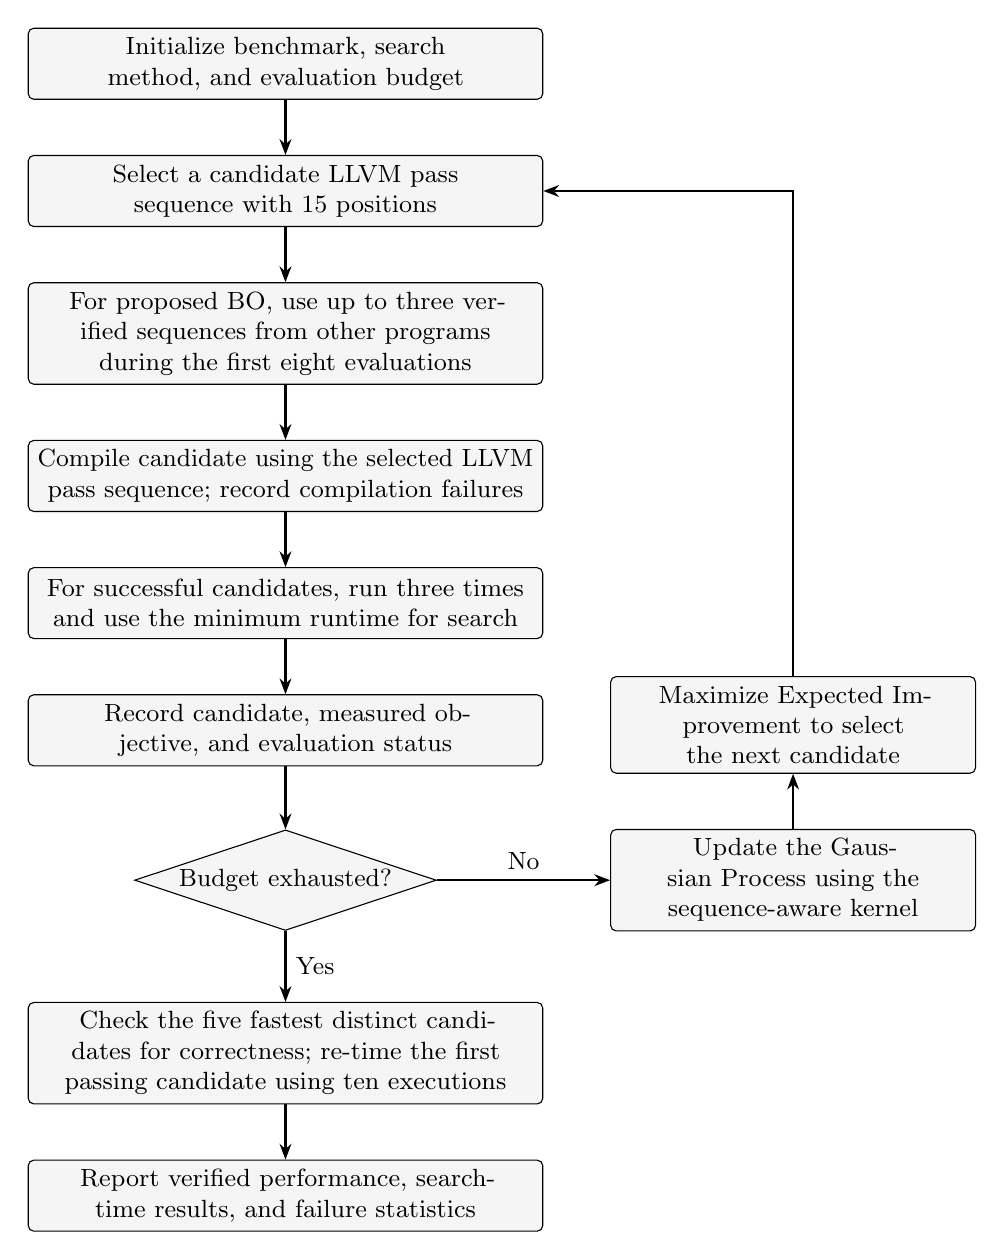
\begin{tikzpicture}[
  node distance=7mm,
  box/.style={draw, rounded corners=2pt, align=center, text width=6.3cm, minimum height=9mm, font=\small, fill=gray!8},
  dec/.style={draw, diamond, aspect=3, align=center, font=\small, inner sep=1pt, fill=gray!8},
  arr/.style={-{Stealth[length=2mm]}, thick}]
\node[box] (a) {Initialize benchmark, search method, and evaluation budget};
\node[box, below=of a] (b) {Select a candidate LLVM pass sequence with 15 positions};
\node[box, below=of b] (c) {For proposed BO, use up to three verified sequences from other programs during the first eight evaluations};
\node[box, below=of c] (d) {Compile candidate using the selected LLVM pass sequence; record compilation failures};
\node[box, below=of d] (e) {For successful candidates, run three times and use the minimum runtime for search};
\node[box, below=of e] (f) {Record candidate, measured objective, and evaluation status};
\node[dec, below=8mm of f] (g) {Budget exhausted?};
\node[box, below=9mm of g] (h) {Check the five fastest distinct candidates for correctness; re-time the first passing candidate using ten executions};
\node[box, below=of h] (i) {Report verified performance, search-time results, and failure statistics};
\node[box, right=2.2cm of g, text width=4.4cm] (j) {Update the Gaussian Process using the sequence-aware kernel};
\node[box, above=of j, text width=4.4cm] (k) {Maximize Expected Improvement to select the next candidate};
\draw[arr] (a)--(b); \draw[arr] (b)--(c); \draw[arr] (c)--(d); \draw[arr] (d)--(e); \draw[arr] (e)--(f); \draw[arr] (f)--(g);
\draw[arr] (g)--node[right, font=\small]{Yes}(h); \draw[arr] (h)--(i);
\draw[arr] (g)--node[above, font=\small]{No}(j); \draw[arr] (j)--(k);
\draw[arr] (k) |- (b);
\end{tikzpicture}}
\caption{Workflow of sequence-aware Bayesian optimization, showing candidate evaluation, Gaussian Process updates, and final correctness verification.}
\label{fig:workflow}
\end{figure*}

\section{Results and Discussion}
\subsection{Verified Speedup}
Table~\ref{tab:verified} reports the verified results. All methods remained below \texttt{-O3} on average: the upper limit of every 95\% confidence interval is below 1. The proposed method (0.942) and TPE (0.952) are statistically indistinguishable: no paired Wilcoxon test of the proposed method against any other method is significant (Table~\ref{tab:wilcoxon}, all $p > 0.3$). Removing the warm start changes neither the speedup (0.933, $p = 0.75$) nor the conclusion, so the warm start does not explain the results. The median verified speedup is between 0.999 and 1.001 for every method, so the selected sequence of a typical run is approximately as fast as \texttt{-O3}; the verified beat rates (44--64\%) count any speedup above 1 without a noise margin and should be read accordingly.

\subsection{Search-Time versus Verified Results}
Table~\ref{tab:search} lists the search-time measures. Selecting the best of 20 candidates, each timed as the minimum of three runs, favors lucky timings: for example, the search-time beat rate of the proposed method is 64\% against a verified beat rate of 44\%, and its best-of-20 geometric-mean speedup (0.956) falls to 0.942 after re-timing. Search-time numbers are therefore reported only as measures of search behavior, not of final performance.

\subsection{Per-Benchmark Results}
Table~\ref{tab:perbench} shows that no method is best on every benchmark. On 2MM and covariance all methods are close to \texttt{-O3}. The proposed method is best on GEMM (0.983) but has a large variance on Floyd--Warshall (standard deviation 0.205), where TPE (0.980) and Random Search (0.960) are better. With five seeds per cell, the standard deviations are indicative only.

\subsection{Failed Builds and Tuning Cost}
Table~\ref{tab:cost} gives the failure rate and the decomposition of tuning time. Executing candidate programs accounts for 84--87\% of the tuning time of every method, while the remainder (model fitting, failed builds, overhead) is only 3--4\%. The lower tuning time of the proposed method (51.6\,s against 64.7--68.1\,s) therefore comes from the execution component: the candidates it evaluated ran faster on average than those of the baselines, not from a cheaper algorithm. Model-fitting time cannot be separated from time lost in failed builds, because failed builds are not timed individually. The proposed method has the lowest failure rate (2.0\%); the variant without warm start is also low (2.8\%).

\subsection{Statistical Comparison}
Table~\ref{tab:wilcoxon} compares the proposed method with each other method on the 25 matched runs. Table~\ref{tab:explore} reports exploratory comparisons of search cost, chosen after inspecting the means. With 18 comparisons the Bonferroni threshold is $0.05/18 \approx 0.0028$. After this correction, two results remain significant: the lower tuning time of both proposed variants against all three baselines, and the lower number of failed builds of the proposed method compared with TPE. The reduction in evaluations needed to beat \texttt{-O3} against TPE ($p = 0.003$) is borderline, and all other differences are not significant. The seeds on one benchmark are not independent, so the $p$-values are somewhat optimistic.

\subsection{Overall Interpretation}
With five seeds and five benchmarks, no method achieves a verified speedup significantly different from the others, and all remain below \texttt{-O3} on average. This is expected for the setting studied: each sequence replaces the \texttt{-O3} pipeline, only 25 passes in 15 positions are available, and the budget is 20 evaluations. The warm start does not change the verified speedup. The measurable differences concern search behavior: the proposed method wasted fewer evaluations on failed builds than TPE and used less time per search than all baselines because its candidates executed faster. These results do not show that the proposed method finds better final sequences than the baselines, and they should be read as an initial comparison under a small budget, not as evidence of general superiority.

\begin{table*}[t]
\caption{Verified results (25 runs per method; correctness checked, minimum of ten timings). Speedups are relative to \texttt{-O3} (higher is better). Robustness is the standard deviation across seeds averaged over benchmarks; the compile-time ratio is relative to \texttt{-O3}.}
\label{tab:verified}
\centering\small
\begin{tabular}{@{}lccccccc@{}}
\toprule
Method & Geometric-mean speedup [95\% CI] & Median & Beat \texttt{-O3} (\%) & Robustness & Compile-time ratio & Valid (\%)\\
\midrule
Random Search & 0.947 [0.906, 0.982] & 0.999 & 44 & 0.065 & 0.931 & 100\\
Genetic Algorithm & 0.917 [0.860, 0.966] & 1.000 & 48 & 0.095 & 0.901 & 100\\
TPE & 0.952 [0.923, 0.977] & 1.000 & 44 & 0.059 & 0.844 & 100\\
Proposed & 0.942 [0.885, 0.981] & 1.000 & 44 & 0.072 & 0.948 & 100\\
Proposed, no warm start & 0.933 [0.876, 0.981] & 1.001 & 64 & 0.097 & 1.107 & 100\\
\bottomrule
\end{tabular}
\end{table*}

\begin{table}[t]
\caption{Search-time results (minimum of three timings, best of 20 evaluations; biased towards favorable timings)}
\label{tab:search}
\centering\footnotesize
\begin{tabular}{@{}lccc@{}}
\toprule
Method & Best-of-20 speedup & Beat \texttt{-O3} (\%) & Evals.\ to beat \texttt{-O3}\\
\midrule
Random Search & 0.954 & 48 & 12.3\\
Genetic Algorithm & 0.928 & 52 & 12.7\\
TPE & 0.945 & 48 & 14.8\\
Proposed & 0.956 & 64 & 9.9\\
Proposed, no warm start & 0.940 & 68 & 10.0\\
\bottomrule
\end{tabular}
\end{table}

\begin{table*}[t]
\caption{Verified speedup per benchmark (mean $\pm$ standard deviation over five seeds)}
\label{tab:perbench}
\centering\small
\begin{tabular}{@{}lccccc@{}}
\toprule
Benchmark & Random & GA & TPE & Proposed & Proposed, no warm start\\
\midrule
2MM & 0.979 $\pm$ 0.049 & 0.979 $\pm$ 0.052 & 0.980 $\pm$ 0.048 & 0.979 $\pm$ 0.048 & 0.979 $\pm$ 0.049\\
Covariance & 0.998 $\pm$ 0.007 & 1.000 $\pm$ 0.003 & 0.983 $\pm$ 0.039 & 1.000 $\pm$ 0.002 & 1.001 $\pm$ 0.001\\
Floyd--Warshall & 0.960 $\pm$ 0.053 & 0.816 $\pm$ 0.213 & 0.980 $\pm$ 0.047 & 0.863 $\pm$ 0.205 & 0.923 $\pm$ 0.176\\
GEMM & 0.963 $\pm$ 0.052 & 0.919 $\pm$ 0.094 & 0.901 $\pm$ 0.083 & 0.983 $\pm$ 0.039 & 0.878 $\pm$ 0.182\\
Jacobi-2D & 0.860 $\pm$ 0.163 & 0.920 $\pm$ 0.111 & 0.925 $\pm$ 0.078 & 0.926 $\pm$ 0.063 & 0.927 $\pm$ 0.076\\
\bottomrule
\end{tabular}
\end{table*}

\begin{table}[t]
\caption{Failed builds and tuning time per search (seconds)}
\label{tab:cost}
\centering\footnotesize
\setlength{\tabcolsep}{3pt}
\begin{tabular}{@{}lcccccc@{}}
\toprule
Method & Failed/search & Failed (\%) & Total & Compile & Execute & Other\\
\midrule
Random Search & 1.12 & 5.6 & 65.1 & 6.3 & 56.8 & 2.0\\
Genetic Algorithm & 0.64 & 3.2 & 64.7 & 6.7 & 56.0 & 2.0\\
TPE & 1.32 & 6.6 & 68.1 & 6.3 & 59.5 & 2.3\\
Proposed & 0.40 & 2.0 & 51.6 & 6.6 & 43.2 & 1.8\\
Proposed, no warm start & 0.56 & 2.8 & 54.4 & 7.2 & 45.5 & 1.7\\
\bottomrule
\end{tabular}
\end{table}

\begin{table}[t]
\caption{Paired Wilcoxon signed-rank test on verified speedup (25 pairs). Difference is proposed minus other, median.}
\label{tab:wilcoxon}
\centering\small
\begin{tabular}{@{}lcc@{}}
\toprule
Comparison & Median difference & $p$\\
\midrule
Proposed vs Random Search & $+0.0001$ & 0.542\\
Proposed vs Genetic Algorithm & $+0.0004$ & 0.560\\
Proposed vs TPE & $+0.0008$ & 0.325\\
Proposed vs no warm start & $-0.0001$ & 0.751\\
\bottomrule
\end{tabular}
\end{table}

\begin{table*}[t]
\caption{Exploratory paired comparisons of search cost (median difference, first method minus second; $p$ from the Wilcoxon signed-rank test; negative differences favor the first method; Bonferroni threshold 0.0028)}
\label{tab:explore}
\centering\small
\begin{tabular}{@{}lcccccc@{}}
\toprule
 & \multicolumn{2}{c}{Evaluations to beat \texttt{-O3}} & \multicolumn{2}{c}{Failed builds} & \multicolumn{2}{c}{Tuning time (s)}\\
\cmidrule(lr){2-3}\cmidrule(lr){4-5}\cmidrule(lr){6-7}
Comparison & Median diff. & $p$ & Median diff. & $p$ & Median diff. & $p$\\
\midrule
Proposed vs Random Search & 0.00 & 0.135 & 0.00 & 0.006 & $-8.63$ & $<0.001$\\
Proposed vs Genetic Algorithm & 0.00 & 0.162 & 0.00 & 0.516 & $-10.67$ & $<0.001$\\
Proposed vs TPE & $-1.00$ & 0.003 & $-1.00$ & $<0.001$ & $-13.93$ & $<0.001$\\
No warm start vs Random Search & 0.00 & 0.262 & 0.00 & 0.035 & $-12.25$ & $<0.001$\\
No warm start vs Genetic Algorithm & 0.00 & 0.179 & 0.00 & 0.848 & $-10.42$ & $<0.001$\\
No warm start vs TPE & $-1.00$ & 0.006 & 0.00 & 0.018 & $-13.20$ & $<0.001$\\
\bottomrule
\end{tabular}
\end{table*}


\section{Limitations and Future Work}
The study has several limitations. First, only five PolyBench/C benchmarks were evaluated on one machine under WSL2, without CPU pinning or frequency control. The CPU model and frequency-governor state were not recorded in the retained experiment metadata, limiting exact hardware-level reproducibility. Second, the search budget was limited to 20 evaluations per run. Although five random seeds were used, this budget may be insufficient to identify high-performing pass sequences, and larger budgets could change the relative performance of the methods. Third, every candidate sequence replaces the LLVM \texttt{-O3} optimization pipeline, and the search space is limited to 25 optimization passes arranged in 15 positions. Applying sequences after \texttt{-O3}, or exploring a larger pass set, was not evaluated. Fourth, only the proposed method used warm-start sequences, selected from other programs within the same evaluated benchmark set rather than from a disjoint external training set. The no-warm-start ablation did not show a meaningful improvement in verified speedup, so these experiments do not establish that warm-start transfer generalizes to unseen programs; this requires a separate benchmark-disjoint evaluation. Fifth, search-time measurements can favor candidates with unusually low observed execution times, and the search-cost comparisons are exploratory. Seeds on the same benchmark may also be correlated. Sixth, the verified beat rate counts any measured speedup above 1 without accounting for a minimum practically meaningful improvement. Seventh, tuning time could not be fully separated into model-fitting time and time spent on failed builds. Finally, executable size was not retained as a primary comparison metric because the size of the complete linked executable includes fixed overhead that may obscure differences attributable to the optimized code.

Future work should evaluate more benchmarks and larger search budgets, investigate sequences applied after \texttt{-O3}, expand the available pass set, and provide equivalent initialization information to competing methods. Further experiments should control CPU frequency and affinity, measure code size using the relevant executable sections, and investigate the relationship between surrogate predictions and verified performance.

\section{Conclusion}
This work investigated sequence-aware Bayesian optimization for LLVM compiler pass ordering and compared it with Random Search, a Genetic Algorithm, Tree-structured Parzen Estimator optimization, and a variant without warm start. The evaluation covered five PolyBench/C benchmarks with a budget of 20 evaluations per search and five random seeds. After correctness checking and re-timing, the proposed method achieved a geometric-mean speedup of 0.942 relative to LLVM \texttt{-O3}, compared with 0.952 for TPE, 0.947 for Random Search, and 0.917 for the Genetic Algorithm. No method achieved a verified geometric-mean speedup above \texttt{-O3}, and paired comparisons did not establish a statistically significant verified-speedup advantage for the proposed method. Removing the warm start did not materially change the conclusion. The proposed method showed lower tuning time and fewer failed evaluations in the reported experiment, but these findings concern search behavior rather than a demonstrated improvement in final program performance. Larger budgets, more benchmarks, and further controlled experiments are required to determine its practical value.

\section*{Code Availability}
The source code and experiment scripts for this study are maintained at \url{https://github.com/shauryaraghav/compiler-pass-ordering/}. The results reported in this manuscript correspond to the experimental protocol described in the paper.

\begin{thebibliography}{30}\small
\bibitem{ashouri2018survey} A. H. Ashouri, W. Killian, J. Cavazos, G. Palermo, and C. Silvano, ``A survey on compiler autotuning using machine learning,'' \textit{ACM Computing Surveys}, vol. 51, no. 5, Art. no. 96, 2018, doi: 10.1145/3197978.
\bibitem{nobre2019nonio} R. Nobre, J. Bispo, T. Carvalho, and J. M. P. Cardoso, ``Nonio---modular automatic compiler phase selection and ordering specialization framework for modern compilers,'' \textit{SoftwareX}, vol. 10, Art. no. 100238, 2019, doi: 10.1016/j.softx.2019.100238.
\bibitem{kruse2020autotuning} M. Kruse, H. Finkel, and X. Wu, ``Autotuning search space for loop transformations,'' in \textit{Proc. IEEE/ACM 6th Workshop on the LLVM Compiler Infrastructure in HPC and Workshop on Hierarchical Parallelism for Exascale Computing}, 2020, doi: 10.1109/LLVMHPCHiPar51896.2020.00007.
\bibitem{queiroz2020hybrid} N. L. Queiroz Junior, A. F. da Silva, and L. G. A. Rodriguez, ``Finding effective compiler optimization sequences: A hybrid approach,'' \textit{Computing and Informatics}, vol. 39, no. 6, pp. 1117--1147, 2020, doi: 10.31577/cai\_2020\_6\_1117.
\bibitem{liu2024dco} J. Liu, J. Fang, T. Wang, J. Xie, C. Huang, and Z. Wang, ``Efficient compiler optimization by modeling passes dependence,'' \textit{CCF Transactions on High Performance Computing}, vol. 6, pp. 588--607, 2024, doi: 10.1007/s42514-024-00197-9.
\bibitem{trofin2021mlgo} M. Trofin, Y. Qian, E. Brevdo, Z. Lin, K. Choromanski, and D. Li, ``MLGO: A machine learning guided compiler optimizations framework,'' arXiv:2101.04808, 2021.
\bibitem{cummins2022compilergym} C. Cummins, B. Wasti, J. Guo, B. Cui, J. Ansel, S. Gomez, S. Jain, J. Liu, O. Teytaud, B. Steiner, Y. Tian, and H. Leather, ``CompilerGym: Robust, performant compiler optimization environments for AI research,'' in \textit{Proc. IEEE/ACM Int. Symp. Code Generation and Optimization}, 2022, pp. 92--105, doi: 10.1109/CGO53902.2022.9741258.
\bibitem{ashouri2024acpo} A. H. Ashouri, M. A. Manzoor, D. M. Vu, R. Zhang, Z. Wang, A. Zhang, B. Chan, T. S. Czajkowski, and Y. Gao, ``Work-in-Progress: ACPO: An AI-Enabled Compiler Framework,'' in \textit{Proc. 2024 Int. Conf. Compilers, Architecture, and Synthesis for Embedded Systems (CASES)}, 2024, p. 21, doi: 10.1109/CASES60062.2024.00011.
\bibitem{hajali2020autophase} A. Haj-Ali, Q. Huang, W. Moses, J. Xiang, K. Asanovic, J. Wawrzynek, and I. Stoica, ``AutoPhase: Juggling HLS phase orderings in random forests with deep reinforcement learning,'' in \textit{Proc. Machine Learning and Systems}, vol. 2, 2020.
\bibitem{wu2020roicf} J. Wu, J. Xu, X. Meng, and Y. Lei, ``A highly reliable compilation optimization passes sequence generation framework,'' \textit{IEICE Trans. Information and Systems}, vol. E103-D, no. 9, pp. 1998--2002, 2020, doi: 10.1587/transinf.2020EDL8006.
\bibitem{jain2022poset} S. Jain, Y. Andaluri, S. VenkataKeerthy, and R. Upadrasta, ``POSET-RL: Phase ordering for optimizing size and execution time using reinforcement learning,'' in \textit{Proc. IEEE Int. Symp. Performance Analysis of Systems and Software}, 2022, pp. 121--131, doi: 10.1109/ISPASS55109.2022.00012.
\bibitem{shahzad2022rl} H. Shahzad, A. Sanaullah, S. Arora, R. Munafo, X. Yao, U. Drepper, and M. Herbordt, ``Reinforcement learning strategies for compiler optimization in high-level synthesis,'' in \textit{Proc. IEEE/ACM Eighth Workshop on the LLVM Compiler Infrastructure in HPC}, 2022, pp. 13--22, doi: 10.1109/LLVM-HPC56686.2022.00007.
\bibitem{pouchet2016polybench} L.-N. Pouchet and T. Yuki, \textit{PolyBench/C 4.2.1: The Polyhedral Benchmark Suite}, 2016. [Online]. Available: \url{https://sourceforge.net/projects/polybench/}.
\bibitem{wu2022bayesian} X. Wu, M. Kruse, P. Balaprakash, H. Finkel, P. Hovland, V. Taylor, and M. Hall, ``Autotuning PolyBench benchmarks with LLVM Clang/Polly loop optimization pragmas using Bayesian optimization,'' \textit{Concurrency and Computation: Practice and Experience}, vol. 34, no. 20, Art. no. e6683, 2022, doi: 10.1002/cpe.6683.
\bibitem{liang2023coreset} Y. Liang, K. Stone, A. Shameli, C. Cummins, M. Elhoushi, J. Guo, B. Steiner, X. Yang, P. Xie, H. Leather, and Y. Tian, ``Learning compiler pass orders using coreset and normalized value prediction,'' in \textit{Proc. 40th Int. Conf. Machine Learning}, Proc. Machine Learning Research, vol. 202, pp. 20746--20762, 2023.
\bibitem{ashouri2022mlgoperf} A. H. Ashouri, M. Elhoushi, Y. Hua, X. Wang, M. A. Manzoor, B. Chan, and Y. Gao, ``Work-in-progress: MLGOPerf: An ML guided inliner to optimize performance,'' in \textit{Proc. Int. Conf. Compilers, Architecture, and Synthesis for Embedded Systems}, 2022, pp. 3--4, doi: 10.1109/CASES55004.2022.00008.
\bibitem{chang2023ensemble} J. Chang and D. Park, ``Work-in-progress: Searching optimal compiler optimization passes sequence for reducing runtime memory profile using ensemble reinforcement learning,'' in \textit{Proc. ACM SIGBED Int. Conf. Embedded Software}, 2023, pp. 3--4, doi: 10.1145/3607890.3608460.
\bibitem{cereda2020collab} S. Cereda, G. Palermo, P. Cremonesi, and S. Doni, ``A collaborative filtering approach for the automatic tuning of compiler optimisations,'' in \textit{Proc. 21st ACM SIGPLAN/SIGBED Conf. Languages, Compilers, and Tools for Embedded Systems}, 2020, pp. 15--25, doi: 10.1145/3372799.3394361.
\bibitem{akiba2019optuna} T. Akiba, S. Sano, T. Yanase, T. Ohta, and M. Koyama, ``Optuna: A next-generation hyperparameter optimization framework,'' in \textit{Proc. 25th ACM SIGKDD Int. Conf. Knowledge Discovery and Data Mining}, 2019, pp. 2623--2631, doi: 10.1145/3292500.3330701.
\bibitem{mammadli2020static} R. Mammadli, A. Jannesari, and F. Wolf, ``Static neural compiler optimization via deep reinforcement learning,'' in \textit{Proc. Sixth Workshop on the LLVM Compiler Infrastructure in HPC}, 2020, pp. 1--11.
\bibitem{venkatakeerthy2020ir2vec} S. VenkataKeerthy, R. Aggarwal, S. Jain, M. S. Desarkar, R. Upadrasta, and Y. N. Srikant, ``IR2Vec: LLVM IR based scalable program embeddings,'' \textit{ACM Trans. Architecture and Code Optimization}, vol. 17, no. 4, Art. no. 32, 2020, doi: 10.1145/3418463.
\bibitem{gibson2022transfer} P. Gibson and J. Cano, ``Transfer-tuning: Reusing auto-schedules for efficient tensor program code generation,'' in \textit{Proc. Int. Conf. Parallel Architectures and Compilation Techniques}, 2022, pp. 28--39, doi: 10.1145/3559009.3569682.
\bibitem{adams2019halide} A. Adams, K. Ma, L. Anderson, R. Baghdadi, T.-M. Li, M. Gharbi, B. Steiner, S. Johnson, K. Fatahalian, F. Durand, and J. Ragan-Kelley, ``Learning to optimize Halide with tree search and random programs,'' \textit{ACM Trans. Graphics}, vol. 38, no. 4, 2019, doi: 10.1145/3306346.3322967.
\bibitem{wang2018mlcompiler} Z. Wang and M. O'Boyle, ``Machine learning in compiler optimization,'' \textit{Proceedings of the IEEE}, vol. 106, no. 11, pp. 1879--1901, 2018, doi: 10.1109/JPROC.2018.2817118.
\bibitem{hajali2021thesis} A. Haj-Ali, \textit{Machine Learning in Compiler Optimization}, Technical Report UCB/EECS-2021-2, University of California, Berkeley, 2021.
\bibitem{cummins2023llmcompiler} C. Cummins, V. Seeker, D. Grubisic, M. Elhoushi, Y. Liang, B. Roziere, J. Gehring, F. Gloeckle, K. Hazelwood, G. Synnaeve, and H. Leather, ``Large language models for compiler optimization,'' arXiv:2309.07062, 2023.
\bibitem{grubisic2024feedback} D. Grubisic, C. Cummins, V. Seeker, and H. Leather, ``Compiler generated feedback for large language models,'' arXiv:2403.14714, 2024.
\bibitem{munafo2023policy} R. Munafo, H. Shahzad, A. Sanaullah, S. Arora, U. Drepper, and M. Herbordt, ``Improved models for policy-agent learning of compiler directives in HLS,'' in \textit{Proc. IEEE High Performance Extreme Computing Conference}, 2023, pp. 1--8, doi: 10.1109/HPEC58863.2023.10363530.
\bibitem{llvm1813notes} LLVM Project, ``LLVM 18.1.3 release notes,'' 2024. [Online]. Available: \url{https://releases.llvm.org/18.1.3/docs/ReleaseNotes.html}.
\bibitem{llvm1813passes} LLVM Project, ``LLVM 18.1.3: LLVM's analysis and transform passes,'' 2024. [Online]. Available: \url{https://releases.llvm.org/18.1.3/docs/Passes.html}.
\end{thebibliography}

\end{document}
